\chapter{Ricevitori 2.0}
\label{capitolo4}
\thispagestyle{empty}
In questo capitolo tratteremo la progettazzione e la realizzazione del nuovo  ricevitore per la ricezione degli allarmi tramite vettori TCP/IP sfruttando sia le normali linee ADSL e GPRS.
\section{Nuovi vettori di comunicazione: dal PSTN al TCP/IP}
Con la diffusione della fibra ottica e delle comunicazione VoIP sono sempre meno le tradizionali linee PSTN che permettono la comunicazione di messaggi tramite i toni. Si è deciso perciò di passare alla comunicazione TCP/IP per comunicare gli eventi di allarme. Questo tipo di comunicazione permette di utilizzare sia connessioni ADSL che connessioni GPRS senza dover modificare nulla per quanto riguarda i protocolli di trasmissione.\\
Per poter utilizzare questa tipo di vettori di comunicazione sono stati adattati due protocolli standard utilizzati normalmente nella comunicazione PSTN per essere trasmetti su canali TCP/IP, questi due protocolli sono:
\begin{itemize}
	\item Contact-ID over IP
	\item SIA over IP
\end{itemize}
Per l'analisi e lo studio del protocollo si è fatto riferimento a due documenti della Security Industry Assocation, questi documenti sono ANSI/SIA DC-09-2007 per la trasmissione di eventi sulla rete internet e AnSI/SIA DC-07-2001 che descrive l'interfaccia di comunicazione.
\section{I protocolli di comunicazione}
I due protocolli di comuncicazione vengo trasmessi nello stesso modo quindi la nostra analisi partirà con la descrizione della struttura del pacchetto per poi descrivere le informazioni trasmette da questo protocollo.
\subsection{La struttura del pacchetto}
Il pacchetto di trasmissione è così formato:
$$
\begin{array}{c}
\langle LF\rangle\langle CRC\rangle\langle 0LLL\rangle\langle ''ID''\rangle\langle Sequence\#\textbf{!}segment\#|\rangle\\\langle\textbf{R}reciver\rangle\langle\textbf{L}line\#\rangle
{[data]}\langle timestamp\rangle \langle CR\rangle\\
\end{array}	 
$$
Dove i campi indicati sono rispettivamente:
\begin{description}
	\item[LF:] indica il carattere esadecimale \texttt{0x0A} e sta ad indicare l'inizio del pacchetto;
	\item[CRC:] campo utilizzato per il controllo degli errori tramite un meccanismo di Cyclic redundancy Check a 16 bit;
	\item[0LLL:] campo utilizzato per indicare la lunghezza del pacchetto. Essa è calcolata considerando come primo carattere le virgolette del campo ID e come ultimo il carattere '$ ] $';
	\item[''ID'':] il campo ID è una stringa che identifica la tipologia di messaggio contenuta nel campo \texttt{data} quelli più importanti per noi sono i tag:
	\begin{itemize}
		\item SIA-DCS,
		\item ADM-CID.
	\end{itemize}
	utilizzati per indicare che il messaggio contenuto nel campo \texttt{data} è un messaggio di allarme con la normale codifica SIA oppure Contact-ID;
	\item[Sequence\#\textbf{!}segment\#:] questo campo è composto da due sotto-campi il primo, \emph{Sequence} è un numero di quattro cifre obbligatorio e serve ad indicare il numero sequenziale del messaggio inviato, se questo valore è seguito dal carattere ''\texttt{!}'' allora è presente un secondo numero utilizzato soprattutto nel caso in cui il messaggio contenuto nel campo \texttt{data} fosse troppo lungo da non poter essere inviato in un solo messaggio;
	\item[\textbf{R}receiver:] questo campo è valore composto da un numero variabile di cifre che precedute dalla lettera \texttt{R} che identificano chi sta trasmettendo, in molti casi questo valore conincide con il codice della centrale;
	\item[\textbf{L}line\#:] campo variabile composto dalla lettera \texttt{L} seguita da 1 a 6 cifre ed indica la linea di ricezione;
	\item[{[...data...]}:] stringa che contiene le informazioni da trasmettere essa è composta da una parentesi quadrata seguita dal numero identificativo della centrale preceduto dal carattere ''\#'' e seguito dal carattere ''\texttt{|}'', dopo questo carattere è presente la vera informazione del messaggio, il delimitatore di fine stringa è una parentesi quadrata chiusa;
	\item[timestamp:] un campo non obbligatorio che indica l'istante in cui il messaggio è stato accodato per l'invio, esso ha la seguente formattazione autoesplicativa
	\begin{center}
		\texttt{\_HH:MM:SS,MM-DD-YYYY}
	\end{center}
	\item[CR:] è il delimitatore finale del pacchetto e corrisponde al carattere ASCII corrispondente al valore esadecimale \texttt{0x0D}			
\end{description}
Con lo standard DC09 viene introdotto anche un campo supplementare tra quello \texttt{data} ed il \texttt{timestamp} questo campo, denominato \texttt{xdata} anchesso compreso tra parentesi quadrata estende la potenza di espressione del protocollo. Il campo \texttt{xdata} inizia sempre con un carattere ASCII maiuscolo compreso nel range ''G'' e ''Z'' il cui significato è mostrato in \tablename \ref{tab:xdata}
\begin{table}
	\begin{tabularx}{\linewidth}{|l|c|X|}
		\hline
		\textbf{Nome} & \textbf{Id} & \textbf{Descrizione} \\
		\hline
		Tempo di occorrenza & ''H'' & Timestamp nel quale si è verificato l'evento\\
		\hline
		MAC Address & ''M'' & Mac address del dispositivo trasmettitore\\
		\hline
		Verifica & ''V'' & Informazioni riguardo ad audio o video associate l'evento\\
		\hline
		Testo di allarme & ''I'' & Breve testo che contiene informazioni riguardanti l'allarme o un commento\\
		\hline
		Nome del sito & ''S'' & Nome del sito nel quale è avvenuto l'allarme\\
		\hline
		Nome dell'edificio & ''O'' & Etichetta che contiene informazioni riguardanti l'edificio che ha generato l'evento.\\
		\hline
		Luogo & ''L'' & Indicazione precisa di dove è avvenuto l'evento segnalato\\
		\hline
		Longitudine & ''X'' & Longitudine del luogo\\
		\hline
		Latitudine & ''Y'' & Latitudine del luogo\\
		\hline
		Altitudine & ''Z'' & Altitudine del luogo\\
		\hline
	\end{tabularx}
	\caption{Possibili valori iniziali per il campo \texttt{xdata}}\label{tab:xdata}
\end{table}
\subsection{La criptazione del pacchetto}
La struttura del pacchetto appena mostrata è utilizzabile così com'è in caso di comunicazione tra una centrale di allarme e un ricevitore in ambiente locale. Tuttavia quando le informazioni devono viaggiare attraverso internet è necessario che le informazioni siano protette in qualche modo. Per fare ciò lo standard DC09 prevede che i pacchetti siano criptati tramite algoritmo di criptazione AES che può utilizzare chiavi a 128, 192 o 256 bits.\\
Tuttavia non viene criptato l'intero pacchetto ma solamente il campo \texttt{data} dello stesso. Per indicare che il pacchetto è criptato si aggiunge il carattere ''*'' prima dell'etichetta nel campo ID.\\
Visto che la criptazione AES richiede che il pacchetto da criptare sia di lunghezza multipla di 16 per rispettare questo vincolo lo standard prevede l'inserimento di un campo \texttt{pad} composto da caratteri random tra il carattere ''['' e il campo account all'interno del campo \texttt{data}.\\
Secondo lo standard è necessario che il software di ricezione implementi la criptazione tramite una qualsiasi delle tre chiavi, tuttavia nel nostro caso abbiamo implementato solo la criptazione con chiave a 128 bit lasciando ad una futura implementazione le altre due chiavi. Questa supposizione è valida in quanto le centrali di un determinato tipo implementano solamente un tipo di criptazione.
\subsection{I tipi di pacchetto}
Dopo aver visto come sono strutturati i pacchetti di informazione vediamo ora quali informazioni possono essere trasmesse da questi pacchetti.
Lo standard prevede una classificazione per le tipologie di pacchetti, in particolare si distinguono tre classi principali:
\begin{itemize}
	\item Event Messages
	\item Supervisor Messages
	\item Acknowledgement Messages
\end{itemize}
Inoltre lo standard DC07 prevede per uno sviluppo futuro dei messaggi di \emph{data/operation request} pensati per essere inviati dal ricevitore per richiede lo svolgimento di alcune operazioni o lo stato di alcuni componenti.
\subsubsection{Event messages}
Gli event messages sono quei messaggi inviati dalla ceentrale di sicurezza per comunicare degli eventi al ricevitore. Essi rispettano lo standard appena descritto, il campo \texttt{ID} di questo tipo di messaggi può essere uno dei seguenti:
\begin{itemize}
	\item SIA-DCS
	\item ADM-CID
	\item SIA-PUL
	\item ACR-SF
	\item ADM-41E
	\item FBI-SF
	\item SK-FSK1
\end{itemize}
tuttavia gli unici tag che noi supporteremo saranno quelli del SIA-DCS e ADM-CID i quali sono anche gli unici obbligatori secondo lo standard.
\subsubsection{Supervisor message}
Questo tipo di messaggi non sono obbligatori, tuttavia sono molto consigliati, in quanto permettono di monitorare periodicamente lo stato della connessione. Questi messaggi sono inviati periodicamente dalla centrale di allarme al ricevitore, il tempo tra una trasmissione e l'altra può essere impostato secondo lo standard da un minimo di 10 secondi ad un massimo di 1080 ore. Se nessun tipo di messaggio raggiunge il ricevitore in questo intervallo di tempo la comunicazione fallisce e il ricevitore dovrebbe segnalare la mancata comunicazione, inoltre, un evento di mancata comunicazione dovrebbe essere registrato dalla centrale.\\
Quando il sistema di supervisione è attivo, periodicamente la centrale invia un messaggio strutturato come in precedenza ma con \texttt{ID} uguale a \emph{NULL} e campo \texttt{data} vuoto. Un esempio di messaggio è il seguente:
$$
\begin{array}{c}
\langle LF\rangle\langle CRC\rangle\langle 0LLL\rangle\langle ''NULL''\rangle\langle 0000\rangle\\\langle\textbf{R}recv\rangle\langle\textbf{L}pref\rangle
{[]}\langle timestamp\rangle \langle CR\rangle\\
\end{array}	 
$$
\subsubsection{Acknowledgment message}
Quando il ricevitore riceve dalla centrale un evento essp deve rispondere con un messaggio che può essere di quattro tipi:
\begin{itemize}
	\item ACK
	\item NAK
	\item DUH
	\item RSP
\end{itemize}
Il messaggio di ACK corrisponde ad una risposta positiva e viene inviato quando il ricevitore riceve correttamente l'evento senza errori, un esempio di messaggio di ACK è il seguente:
$$
\begin{array}{c}
\langle LF\rangle\langle CRC\rangle\langle 0LLL\rangle\langle ''ACK''\rangle\langle seq\rangle\\\langle\textbf{R}recv\rangle\langle\textbf{L}pref\rangle
{[]}\langle timestamp\rangle \langle CR\rangle\\
\end{array}	 
$$
dove i campi \texttt{seq}, \texttt{recv} e \texttt{pref} vengono copiati dal messaggio originale al quale si vuole dare una risposta.\\
Il messaggio di NAK è simile a quello di ACK tuttavia cambia il campo \texttt{ID} e il numero di \texttt{seq} che viene impostato a 0000, un esempio è riportato di seguito.
$$
\begin{array}{c}
\langle LF\rangle\langle CRC\rangle\langle 0LLL\rangle\langle ''NAK''\rangle\langle 0000\rangle\\\langle\textbf{R}recv\rangle\langle\textbf{L}pref\rangle
{[]}\langle timestamp\rangle \langle CR\rangle\\
\end{array}	 
$$
Il pacchetto DUH viene inviato nel caso in cui il ricevitore, pur avendo verificato che il pacchetto è formattato correttamente e non contiene errori, non è in grado di tradurlo o comunque di interpretare la richiesta. In questo caso i campi \texttt{seq}, \texttt{recv} e \texttt{pref} sono uguali a quelli della richiesta ricevuta.\\
Il pacchetto RSP è stato introdotto come pacchetto di risposta per i messaggi di data/operation request tuttavia come questi pacchetti è pensato per un uso futuro. A differenza dei pacchetti precedenti il campo \texttt{data} contiene dei valori. Il numero di sequenza, del ricevitore e della linea sono copiati dal pacchetto di richiesta.
\subsection{La connessione}
Lo standard DC09 prevede che la connessione tra il ricevitore e la centrale possa avvenire sia tramite l'utilizzo dello \emph{User Data Protocol} (UDP) sia tramite l'utilizzo del \emph{Transmission Control Protol} (TCP), il ricevitore da noi implementato permette attualmente solo l'utilizzo della modalità TCP, in quanto la modalità UDP è meno diffusa ed implementata tramite hardware con una scheda di espansione per il ricevitore System III.\\
Da notare il fatto che per la trasmissione tramite UDP nell'header del messaggio è necessario introdurre la porta della centrale d'allarme sulla quale il ricevitore dovrà inviare la risposta al messaggio.
In \figurename \ref{fig:transmission} vediamo la sequenza di messaggi che avviene durante la trasmissione di un evento.
\begin{figure}
	\centering
	\subfigure[]
	{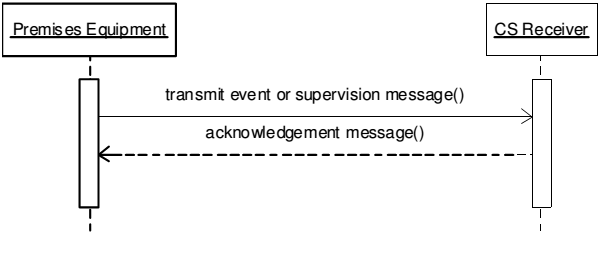
\includegraphics[width=7cm]{pictures/udp.png}\label{fig:udp}}
	\hspace{5mm}
	\subfigure[]
	{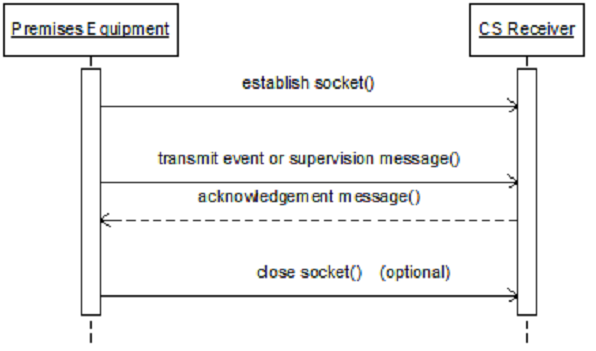
\includegraphics[width=6.5cm]{pictures/tcp.png}\label{fig:tcp}}
	\caption{Esempio di trasmissione UDP \ref{fig:udp} e TCP \ref{fig:tcp} }\label{fig:transmission}
\end{figure}
\section{La struttura dati}
Come abbiamo detto nel \chaptername \ref{capitolo3} uno dei nostri obiettivi è quello di mantenere la retrocompatibilità con il vecchio software di Lis fino al completo aggiornamento dei moduli. Per fare ciò è stato necessario mantenere la struttura dati precedente per far si che il resto del software potesse prelevare i dati senza nessuna complicazione. In particolare la tabella più importante per la ricezione degli eventi era quella \texttt{allarmi\_contact\_id} i cui campi si ricavano dallo script di creazione del \lstname \ref{lst:allarmicontactid}
\begin{lstlisting}[language=SQL,caption=Tabella allarmi\_contact\_id,label=lst:allarmicontactid]
CREATE TABLE allarmi_contact_id
(
	ac_id integer NOT NULL DEFAULT nextval(('"allarmi_contact_id_seq"'::text)::regclass),
	ac_centrale character varying(20),
	ac_allarme character varying(10),
	ac_area bigint,
	ac_zona bigint,
	ac_giorno smallint,
	ac_mese smallint,
	ac_anno smallint,
	ac_ora smallint,
	ac_minuto smallint,
	ac_secondo smallint,
	ac_data_inserimento timestamp without time zone DEFAULT now(),
	ac_pending character(1) DEFAULT 's'::character varying,
	ac_porta_seriale integer,
	ac_n_ricevitore smallint,
	ac_n_gruppo smallint,
	CONSTRAINT allarmi_contact_id_pkey PRIMARY KEY (ac_id)
)
\end{lstlisting}
Come si nota i campi da compilare sono diversi anche se non tutti necessari. Il campo allarme contiene il codice Contact ID dell'allarme ricevuto, nel paragrafo successivo vedremo come questo meccanismo sia stato adattato per l'utilizzo anche dei codici di allarme SIA. Il campo \texttt{pending} serve al cp200\_4 per identificare quali allarmi sono già stati processati in quanto questa tabella mantiene anche lo storico giornaliero degli allarmi ricevuti.\\
Oltre a questa tabella si è deciso anche di aggiornare una serie di tabelle collegate tra loro che hanno la funzione di monitorare lo stato dei ricevitori. Nel vecchio software per verificare la corretta esecuzione del software, ogni qualvolta che una segnalazione giungeva ad uno dei ricevitori veniva aggiornato un campo nella tabella \texttt{seriale} il quale è collegato alla tabella \texttt{ricevitori}; questo collegamento è mostrato in \figurename \ref{fig:erricevitori}.
Il codice di creazione di queste tabelle è mostrato nel \lstname \ref{lst:ricevitori}.
\begin{figure}
	\centering
	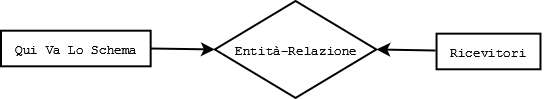
\includegraphics[width=0.7\linewidth]{pictures/erricevitori.png}
	\caption{Schema relazionale delle tabelle che controllano i ricevitori}\label{fig:erricevitori}
\end{figure}
\begin{lstlisting}[language=SQL,caption=Tabelle ricevitori,label=lst:ricevitori]
CREATE TABLE seriale
(
	se_id integer NOT NULL DEFAULT 		nextval(('"seriale_se_id_seq"'::text)::regclass),
	se_numero integer,
	se_stato character varying(1) DEFAULT 's'::character varying,
	se_allarme integer,
	se_controllo character varying(1),
	CONSTRAINT pk_seriale PRIMARY KEY (se_id)
)

CREATE TABLE ricevitore
(
	ri_id integer NOT NULL DEFAULT 	nextval(('"ricevitore_ri_id_seq"'::text)::regclass),
	se_id integer,
	ri_stato character varying(2) DEFAULT 'n'::character varying,
	ri_tipo character varying(50),
	ri_batteria smallint,
	ri_modalita smallint,
	ri_mancanza_220 smallint,
	ri_stampante smallint,
	ri_collegato smallint,
	ri_data_220 timestamp with time zone,
	ri_data_batteria timestamp with time zone,
	ri_stato_ricevitore smallint,
	ri_numero smallint,
	CONSTRAINT pk_ricevitore PRIMARY KEY (ri_id),
	CONSTRAINT fk_ricevito_reference_seriale FOREIGN KEY (se_id)
	REFERENCES seriale (se_id) MATCH SIMPLE
	ON UPDATE RESTRICT ON DELETE RESTRICT
)
\end{lstlisting}
Questa meccanismo se pur non necessario per il corretto funzionamento del vecchio software è stato mantenuto, con dei piccoli adattamenti, per monitorare il funzionamento del nuovo software di ricezione.
Tuttavia come si nota dalla complessità delle tabelle questo sistema porta con se anche degli elementi caratteristici del passato come l'utilizzo di una tabella \texttt{SERIALE} utilizzata dai tempi in cui i ricevitori erano ancora collegati tramite questo tipo di connessione cablata.

\section{Architettura del sistema}
Analizziamo ora come è stato sviluppato il sistema. Si è deciso di passare ad un softwre strutturato per classi. L'idea era quella di avere un controllore che monitorasse periodicamente i diversi ricevitori e nel caso questi non fossero avviati li riavviasse in automatico. I ricevitori dal canto loro dovevano comportarsi tutti pressochè alla stessa maniera ovvero le funzioni principali che dovevano svolgere erano quella di aggiornare il campo \texttt{controllo} della tabella seriale e caricare l'allarme sul database rispettando lo standard Contact-ID.
\section{Implementazione}
Inanzitutto si è deciso di sviluppare il software in linguaggio C++ aggiornato allo standard 0x rilasciato nel 2011 per supportare meglio il multi-threading e per fare ciò si è deciso di utilizzare il compilatore gcc-4.8 l'ultimo rilasciato al momento dell'implementazione